
%% bare_jrnl.tex
%% V1.3
%% 2007/01/11
%% by Michael Shell
%% see http://www.michaelshell.org/
%% for current contact information.
%%
%% This is a skeleton file demonstrating the use of IEEEtran.cls
%% (requires IEEEtran.cls version 1.7 or later) with an IEEE journal paper.
%%
%% Support sites:
%% http://www.michaelshell.org/tex/ieeetran/
%% http://www.ctan.org/tex-archive/macros/latex/contrib/IEEEtran/
%% and
%% http://www.ieee.org/



% *** Authors should verify (and, if needed, correct) their LaTeX system  ***
% *** with the testflow diagnostic prior to trusting their LaTeX platform ***
% *** with production work. IEEE's font choices can trigger bugs that do  ***
% *** not appear when using other class files.                            ***
% The testflow support page is at:
% http://www.michaelshell.org/tex/testflow/


%%*************************************************************************
%% Legal Notice:
%% This code is offered as-is without any warranty either expressed or
%% implied; without even the implied warranty of MERCHANTABILITY or
%% FITNESS FOR A PARTICULAR PURPOSE!
%% User assumes all risk.
%% In no event shall IEEE or any contributor to this code be liable for
%% any damages or losses, including, but not limited to, incidental,
%% consequential, or any other damages, resulting from the use or misuse
%% of any information contained here.
%%
%% All comments are the opinions of their respective authors and are not
%% necessarily endorsed by the IEEE.
%%
%% This work is distributed under the LaTeX Project Public License (LPPL)
%% ( http://www.latex-project.org/ ) version 1.3, and may be freely used,
%% distributed and modified. A copy of the LPPL, version 1.3, is included
%% in the base LaTeX documentation of all distributions of LaTeX released
%% 2003/12/01 or later.
%% Retain all contribution notices and credits.
%% ** Modified files should be clearly indicated as such, including  **
%% ** renaming them and changing author support contact information. **
%%
%% File list of work: IEEEtran.cls, IEEEtran_HOWTO.pdf, bare_adv.tex,
%%                    bare_conf.tex, bare_jrnl.tex, bare_jrnl_compsoc.tex
%%*************************************************************************

% Note that the a4paper option is mainly intended so that authors in
% countries using A4 can easily print to A4 and see how their papers will
% look in print - the typesetting of the document will not typically be
% affected with changes in paper size (but the bottom and side margins will).
% Use the testflow package mentioned above to verify correct handling of
% both paper sizes by the user's LaTeX system.
%
% Also note that the "draftcls" or "draftclsnofoot", not "draft", option
% should be used if it is desired that the figures are to be displayed in
% draft mode.
%
\documentclass[journal]{IEEEtran}
\usepackage{graphicx}
\usepackage{amssymb}
\usepackage{url}
\usepackage{breakurl}
\def\UrlBreaks{\do\/\do-}
%
% If IEEEtran.cls has not been installed into the LaTeX system files,
% manually specify the path to it like:
% \documentclass[journal]{../sty/IEEEtran}





% Some very useful LaTeX packages include:
% (uncomment the ones you want to load)


% *** MISC UTILITY PACKAGES ***
%
%\usepackage{ifpdf}
% Heiko Oberdiek's ifpdf.sty is very useful if you need conditional
% compilation based on whether the output is pdf or dvi.
% usage:
% \ifpdf
%   % pdf code
% \else
%   % dvi code
% \fi
% The latest version of ifpdf.sty can be obtained from:
% http://www.ctan.org/tex-archive/macros/latex/contrib/oberdiek/
% Also, note that IEEEtran.cls V1.7 and later provides a builtin
% \ifCLASSINFOpdf conditional that works the same way.
% When switching from latex to pdflatex and vice-versa, the compiler may
% have to be run twice to clear warning/error messages.






% *** CITATION PACKAGES ***
%
%\usepackage{cite}
% cite.sty was written by Donald Arseneau
% V1.6 and later of IEEEtran pre-defines the format of the cite.sty package
% \cite{} output to follow that of IEEE. Loading the cite package will
% result in citation numbers being automatically sorted and properly
% "compressed/ranged". e.g., [1], [9], [2], [7], [5], [6] without using
% cite.sty will become [1], [2], [5]--[7], [9] using cite.sty. cite.sty's
% \cite will automatically add leading space, if needed. Use cite.sty's
% noadjust option (cite.sty V3.8 and later) if you want to turn this off.
% cite.sty is already installed on most LaTeX systems. Be sure and use
% version 4.0 (2003-05-27) and later if using hyperref.sty. cite.sty does
% not currently provide for hyperlinked citations.
% The latest version can be obtained at:
% http://www.ctan.org/tex-archive/macros/latex/contrib/cite/
% The documentation is contained in the cite.sty file itself.






% *** GRAPHICS RELATED PACKAGES ***
%
\ifCLASSINFOpdf
  % \usepackage[pdftex]{graphicx}
  % declare the path(s) where your graphic files are
  % \graphicspath{{../pdf/}{../jpeg/}}
  % and their extensions so you won't have to specify these with
  % every instance of \includegraphics
  % \DeclareGraphicsExtensions{.pdf,.jpeg,.png}
\else
  % or other class option (dvipsone, dvipdf, if not using dvips). graphicx
  % will default to the driver specified in the system graphics.cfg if no
  % driver is specified.
  %\usepackage[dvips]{graphicx}
  % declare the path(s) where your graphic files are
  % \graphicspath{{../eps/}}
  % and their extensions so you won't have to specify these with
  % every instance of \includegraphics
  % \DeclareGraphicsExtensions{.eps}
\fi
% graphicx was written by David Carlisle and Sebastian Rahtz. It is
% required if you want graphics, photos, etc. graphicx.sty is already
% installed on most LaTeX systems. The latest version and documentation can
% be obtained at:
% http://www.ctan.org/tex-archive/macros/latex/required/graphics/
% Another good source of documentation is "Using Imported Graphics in
% LaTeX2e" by Keith Reckdahl which can be found as epslatex.ps or
% epslatex.pdf at: http://www.ctan.org/tex-archive/info/
%
% latex, and pdflatex in dvi mode, support graphics in encapsulated
% postscript (.eps) format. pdflatex in pdf mode supports graphics
% in .pdf, .jpeg, .png and .mps (metapost) formats. Users should ensure
% that all non-photo figures use a vector format (.eps, .pdf, .mps) and
% not a bitmapped formats (.jpeg, .png). IEEE frowns on bitmapped formats
% which can result in "jaggedy"/blurry rendering of lines and letters as
% well as large increases in file sizes.
%
% You can find documentation about the pdfTeX application at:
% http://www.tug.org/applications/pdftex





% *** MATH PACKAGES ***
%
%\usepackage[cmex10]{amsmath}
% A popular package from the American Mathematical Society that provides
% many useful and powerful commands for dealing with mathematics. If using
% it, be sure to load this package with the cmex10 option to ensure that
% only type 1 fonts will utilized at all point sizes. Without this option,
% it is possible that some math symbols, particularly those within
% footnotes, will be rendered in bitmap form which will result in a
% document that can not be IEEE Xplore compliant!
%
% Also, note that the amsmath package sets \interdisplaylinepenalty to 10000
% thus preventing page breaks from occurring within multiline equations. Use:
%\interdisplaylinepenalty=2500
% after loading amsmath to restore such page breaks as IEEEtran.cls normally
% does. amsmath.sty is already installed on most LaTeX systems. The latest
% version and documentation can be obtained at:
% http://www.ctan.org/tex-archive/macros/latex/required/amslatex/math/





% *** SPECIALIZED LIST PACKAGES ***
%
%\usepackage{algorithmic}
% algorithmic.sty was written by Peter Williams and Rogerio Brito.
% This package provides an algorithmic environment fo describing algorithms.
% You can use the algorithmic environment in-text or within a figure
% environment to provide for a floating algorithm. Do NOT use the algorithm
% floating environment provided by algorithm.sty (by the same authors) or
% algorithm2e.sty (by Christophe Fiorio) as IEEE does not use dedicated
% algorithm float types and packages that provide these will not provide
% correct IEEE style captions. The latest version and documentation of
% algorithmic.sty can be obtained at:
% http://www.ctan.org/tex-archive/macros/latex/contrib/algorithms/
% There is also a support site at:
% http://algorithms.berlios.de/index.html
% Also of interest may be the (relatively newer and more customizable)
% algorithmicx.sty package by Szasz Janos:
% http://www.ctan.org/tex-archive/macros/latex/contrib/algorithmicx/




% *** ALIGNMENT PACKAGES ***
%
%\usepackage{array}
% Frank Mittelbach's and David Carlisle's array.sty patches and improves
% the standard LaTeX2e array and tabular environments to provide better
% appearance and additional user controls. As the default LaTeX2e table
% generation code is lacking to the point of almost being broken with
% respect to the quality of the end results, all users are strongly
% advised to use an enhanced (at the very least that provided by array.sty)
% set of table tools. array.sty is already installed on most systems. The
% latest version and documentation can be obtained at:
% http://www.ctan.org/tex-archive/macros/latex/required/tools/


%\usepackage{mdwmath}
%\usepackage{mdwtab}
% Also highly recommended is Mark Wooding's extremely powerful MDW tools,
% especially mdwmath.sty and mdwtab.sty which are used to format equations
% and tables, respectively. The MDWtools set is already installed on most
% LaTeX systems. The lastest version and documentation is available at:
% http://www.ctan.org/tex-archive/macros/latex/contrib/mdwtools/


% IEEEtran contains the IEEEeqnarray family of commands that can be used to
% generate multiline equations as well as matrices, tables, etc., of high
% quality.


%\usepackage{eqparbox}
% Also of notable interest is Scott Pakin's eqparbox package for creating
% (automatically sized) equal width boxes - aka "natural width parboxes".
% Available at:
% http://www.ctan.org/tex-archive/macros/latex/contrib/eqparbox/





% *** SUBFIGURE PACKAGES ***
%\usepackage[tight,footnotesize]{subfigure}
% subfigure.sty was written by Steven Douglas Cochran. This package makes it
% easy to put subfigures in your figures. e.g., "Figure 1a and 1b". For IEEE
% work, it is a good idea to load it with the tight package option to reduce
% the amount of white space around the subfigures. subfigure.sty is already
% installed on most LaTeX systems. The latest version and documentation can
% be obtained at:
% http://www.ctan.org/tex-archive/obsolete/macros/latex/contrib/subfigure/
% subfigure.sty has been superceeded by subfig.sty.



%\usepackage[caption=false]{caption}
%\usepackage[font=footnotesize]{subfig}
% subfig.sty, also written by Steven Douglas Cochran, is the modern
% replacement for subfigure.sty. However, subfig.sty requires and
% automatically loads Axel Sommerfeldt's caption.sty which will override
% IEEEtran.cls handling of captions and this will result in nonIEEE style
% figure/table captions. To prevent this problem, be sure and preload
% caption.sty with its "caption=false" package option. This is will preserve
% IEEEtran.cls handing of captions. Version 1.3 (2005/06/28) and later
% (recommended due to many improvements over 1.2) of subfig.sty supports
% the caption=false option directly:
%\usepackage[caption=false,font=footnotesize]{subfig}
%
% The latest version and documentation can be obtained at:
% http://www.ctan.org/tex-archive/macros/latex/contrib/subfig/
% The latest version and documentation of caption.sty can be obtained at:
% http://www.ctan.org/tex-archive/macros/latex/contrib/caption/




% *** FLOAT PACKAGES ***
%
%\usepackage{fixltx2e}
% fixltx2e, the successor to the earlier fix2col.sty, was written by
% Frank Mittelbach and David Carlisle. This package corrects a few problems
% in the LaTeX2e kernel, the most notable of which is that in current
% LaTeX2e releases, the ordering of single and double column floats is not
% guaranteed to be preserved. Thus, an unpatched LaTeX2e can allow a
% single column figure to be placed prior to an earlier double column
% figure. The latest version and documentation can be found at:
% http://www.ctan.org/tex-archive/macros/latex/base/



%\usepackage{stfloats}
% stfloats.sty was written by Sigitas Tolusis. This package gives LaTeX2e
% the ability to do double column floats at the bottom of the page as well
% as the top. (e.g., "\begin{figure*}[!b]" is not normally possible in
% LaTeX2e). It also provides a command:
%\fnbelowfloat
% to enable the placement of footnotes below bottom floats (the standard
% LaTeX2e kernel puts them above bottom floats). This is an invasive package
% which rewrites many portions of the LaTeX2e float routines. It may not work
% with other packages that modify the LaTeX2e float routines. The latest
% version and documentation can be obtained at:
% http://www.ctan.org/tex-archive/macros/latex/contrib/sttools/
% Documentation is contained in the stfloats.sty comments as well as in the
% presfull.pdf file. Do not use the stfloats baselinefloat ability as IEEE
% does not allow \baselineskip to stretch. Authors submitting work to the
% IEEE should note that IEEE rarely uses double column equations and
% that authors should try to avoid such use. Do not be tempted to use the
% cuted.sty or midfloat.sty packages (also by Sigitas Tolusis) as IEEE does
% not format its papers in such ways.


%\ifCLASSOPTIONcaptionsoff
%  \usepackage[nomarkers]{endfloat}
% \let\MYoriglatexcaption\caption
% \renewcommand{\caption}[2][\relax]{\MYoriglatexcaption[#2]{#2}}
%\fi
% endfloat.sty was written by James Darrell McCauley and Jeff Goldberg.
% This package may be useful when used in conjunction with IEEEtran.cls'
% captionsoff option. Some IEEE journals/societies require that submissions
% have lists of figures/tables at the end of the paper and that
% figures/tables without any captions are placed on a page by themselves at
% the end of the document. If needed, the draftcls IEEEtran class option or
% \CLASSINPUTbaselinestretch interface can be used to increase the line
% spacing as well. Be sure and use the nomarkers option of endfloat to
% prevent endfloat from "marking" where the figures would have been placed
% in the text. The two hack lines of code above are a slight modification of
% that suggested by in the endfloat docs (section 8.3.1) to ensure that
% the full captions always appear in the list of figures/tables - even if
% the user used the short optional argument of \caption[]{}.
% IEEE papers do not typically make use of \caption[]'s optional argument,
% so this should not be an issue. A similar trick can be used to disable
% captions of packages such as subfig.sty that lack options to turn off
% the subcaptions:
% For subfig.sty:
% \let\MYorigsubfloat\subfloat
% \renewcommand{\subfloat}[2][\relax]{\MYorigsubfloat[]{#2}}
% For subfigure.sty:
% \let\MYorigsubfigure\subfigure
% \renewcommand{\subfigure}[2][\relax]{\MYorigsubfigure[]{#2}}
% However, the above trick will not work if both optional arguments of
% the \subfloat/subfig command are used. Furthermore, there needs to be a
% description of each subfigure *somewhere* and endfloat does not add
% subfigure captions to its list of figures. Thus, the best approach is to
% avoid the use of subfigure captions (many IEEE journals avoid them anyway)
% and instead reference/explain all the subfigures within the main caption.
% The latest version of endfloat.sty and its documentation can obtained at:
% http://www.ctan.org/tex-archive/macros/latex/contrib/endfloat/
%
% The IEEEtran \ifCLASSOPTIONcaptionsoff conditional can also be used
% later in the document, say, to conditionally put the References on a
% page by themselves.





% *** PDF, URL AND HYPERLINK PACKAGES ***
%
%\usepackage{url}
% url.sty was written by Donald Arseneau. It provides better support for
% handling and breaking URLs. url.sty is already installed on most LaTeX
% systems. The latest version can be obtained at:
% http://www.ctan.org/tex-archive/macros/latex/contrib/misc/
% Read the url.sty source comments for usage information. Basically,
% \url{my_url_here}.





% *** Do not adjust lengths that control margins, column widths, etc. ***
% *** Do not use packages that alter fonts (such as pslatex).         ***
% There should be no need to do such things with IEEEtran.cls V1.6 and later.
% (Unless specifically asked to do so by the journal or conference you plan
% to submit to, of course. )


% correct bad hyphenation here
\hyphenation{op-tical net-works semi-conduc-tor}


\begin{document}
%
% paper title
% can use linebreaks \\ within to get better formatting as desired
\title{Machine Learning Assisted Cognitive Radio}
%
%
% author names and IEEE memberships
% note positions of commas and nonbreaking spaces ( ~ ) LaTeX will not break
% a structure at a ~ so this keeps an author's name from being broken across
% two lines.
% use \thanks{} to gain access to the first footnote area
% a separate \thanks must be used for each paragraph as LaTeX2e's \thanks
% was not built to handle multiple paragraphs
%

\author{Zhikun Zhu, 29356822
\thanks{Zhikun Zhu is with the Department
of Electrical and Computer Science, University of Southampton, Southampton,
UK, SO17 1BJ  e-mail: \textsl{zz1u17@soton.ac.uk}}}

% note the % following the last \IEEEmembership and also \thanks -
% these prevent an unwanted space from occurring between the last author name
% and the end of the author line. i.e., if you had this:
%
% \author{....lastname \thanks{...} \thanks{...} }
%                     ^------------^------------^----Do not want these spaces!
%
% a space would be appended to the last name and could cause every name on that
% line to be shifted left slightly. This is one of those "LaTeX things". For
% instance, "\textbf{A} \textbf{B}" will typeset as "A B" not "AB". To get
% "AB" then you have to do: "\textbf{A}\textbf{B}"
% \thanks is no different in this regard, so shield the last } of each \thanks
% that ends a line with a % and do not let a space in before the next \thanks.
% Spaces after \IEEEmembership other than the last one are OK (and needed) as
% you are supposed to have spaces between the names. For what it is worth,
% this is a minor point as most people would not even notice if the said evil
% space somehow managed to creep in.



% The paper headers
\markboth{~ELEC 6211: Research review}%
{Machine Learning Asisted Cognitive Radios }
% The only time the second header will appear is for the odd numbered pages
% after the title page when using the twoside option.
%
% *** Note that you probably will NOT want to include the author's ***
% *** name in the headers of peer review papers.                   ***
% You can use \ifCLASSOPTIONpeerreview for conditional compilation here if
% you desire.




% If you want to put a publisher's ID mark on the page you can do it like
% this:
%\IEEEpubid{0000--0000/00\$00.00~\copyright~2007 IEEE}
% Remember, if you use this you must call \IEEEpubidadjcol in the second
% column for its text to clear the IEEEpubid mark.



% use for special paper notices
%\IEEEspecialpapernotice{(Invited Paper)}




% make the title area
\maketitle


\begin{abstract}
%\boldmath
$\mathcal N$
This survey paper characterizes the architecture and learning problems in cognitive radio (CR) as well as the significance of implementing artificial intelligence (AI) to solve such problems. Three main categories of machine learning (ML) technique and there working scenario have been discussed, and several implementations of ML to CR systems have also been introduced with their relative merits. In the conclusion, some considerations about future work are summarized.
\end{abstract}
% IEEEtran.cls defaults to using nonbold math in the Abstract.
% This preserves the distinction between vectors and scalars. However,
% if the journal you are submitting to favors bold math in the abstract,
% then you can use LaTeX's standard command \boldmath at the very start
% of the abstract to achieve this. Many IEEE journals frown on math
% in the abstract anyway.

% Note that keywords are not normally used for peerreview papers.
\begin{IEEEkeywords}
Artificial intelligence (AI), cognitive Radio (CR), machine learning, artificial neural network (ANN), support vector machine (SVM), reinforcement learning.
\end{IEEEkeywords}






% For peer review papers, you can put extra information on the cover
% page as needed:
% \ifCLASSOPTIONpeerreview
% \begin{center} \bfseries EDICS Category: 3-BBND \end{center}
% \fi
%
% For peerreview papers, this IEEEtran command inserts a page break and
% creates the second title. It will be ignored for other modes.
\IEEEpeerreviewmaketitle



\section{Introduction and motivation}
% The very first letter is a 2 line initial drop letter followed
% by the rest of the first word in caps.
%
% form to use if the first word consists of a single letter:
% \IEEEPARstart{A}{demo} file is ....
%
% form to use if you need the single drop letter followed by
% normal text (unknown if ever used by IEEE):
% \IEEEPARstart{A}{}demo file is ....
%
% Some journals put the first two words in caps:
% \IEEEPARstart{T}{his demo} file is ....
%
% Here we have the typical use of a "T" for an initial drop letter
% and "HIS" in caps to complete the first word.
\IEEEPARstart{T}{he} term cognitive radio (CR) is initially been introduced in \cite{mitola1999cognitive}, which refers to radio devices that are capable of sensing and adapting to their environment.  Despite various detailed definitions have been proposed, a CR is a software defined radio (SDR) which can automatically adjust its parameters (i.e. modulation, carrier frequency) to adapt to the environment by measuring and decision-making process. Haykin \cite{haykin2005cognitive} envisioned a CR to be `\textsl{an intelligent wireless communication system that is aware of its environment and uses the methodology of understanding-by-building to learn from the environment and adapt to statistical variations in the input stimuli}'. CR aims to achieve two objectives: 1) permanent reliable communications in any RF band, at any location \cite{bkassiny2013survey}; 2) efficient utilization of frequency spectrum resources.


As the dramatic popularity of wireless applications, RF spectrum is getting crowded. However, there are papers pointed out the low-efficiency usage of authorized radio spectrum: in the range from 30 MHz to 3.95 GHz, the average radio spectrum usage in New York City and Chicago are 13.1\% and 17.4\% respectively \cite{mchenry2006chicago}. This average usage becomes 4.54\% in Singapore where some frequency bands are heavily used whereas almost silence for the others \cite{islam2008spectrum}.
\section{Attributes and tasks of cognitive radio}
To explore the efficient utilization methods of radio spectrum, the term \textsl{spectrum holes} is defined in \cite{haykin2005cognitive} as the spectrum band that allocated to the primary users which are unused at specific time and location. The spectrum efficiency could be tremendously improved if a secondary user (cognitive user) can access the spectrum holes. Thus, the main aim for CR is to exploit the spectrum holes. To achieve such goal, a CR is expected to have following properties \cite{he2010survey}:
\begin{enumerate}
  \item Observation: Collect information of the RF environment.
  \item Reconfiguration: Adjust the radio parameters.
  \item Cognition: Understand the information from observation and capability of
the radio (awareness), make decisions on actions (reasoning) as well as learn the relationship between action and performance of the CR (learning).
\end{enumerate}

This set of properties contribute to the scheme of CR, which defined as cognitive cycle \cite{mitola1999cognitive} as shown in Fig. \ref{CognitiveCycle}.
\begin{figure}[!t]
  \centering
  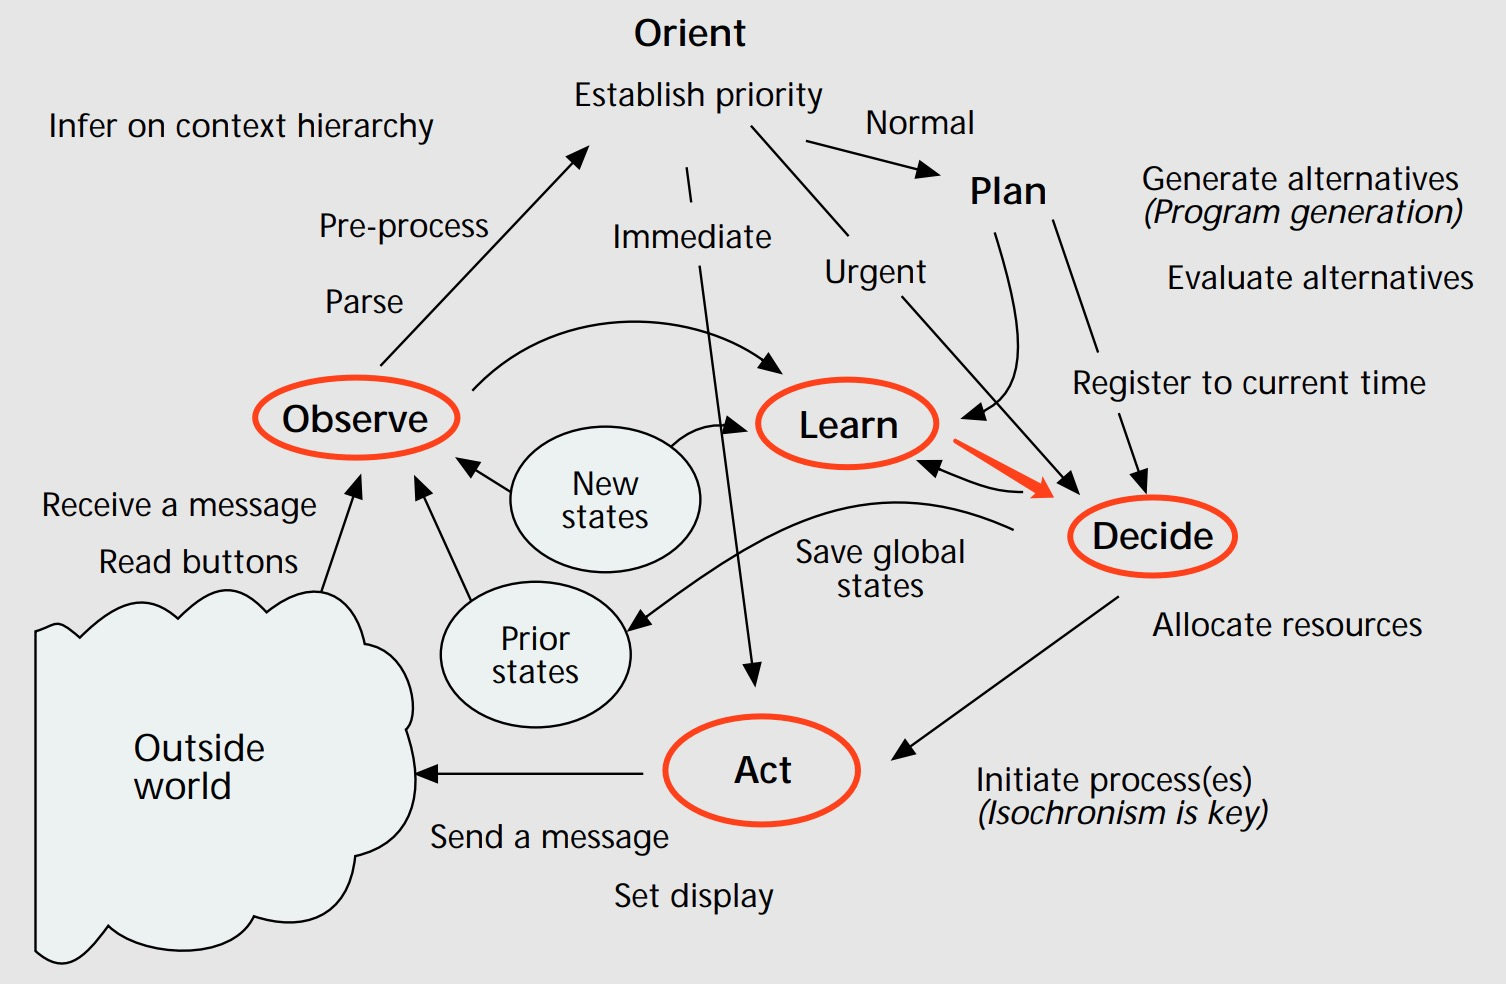
\includegraphics[width=0.5\textwidth]{cogCycle.jpeg}
  % where an .eps filename suffix will be assumed under latex,
  % and a .pdf suffix will be assumed for pdflatex; or what has been declared
  % via \DeclareGraphicsExtensions.
  \caption{The cognition cycle of an autonomous cognitive radio \cite{mitola1999cognitive}. The original cycle in this reference hasn't point out the influence of learning on decision process, where \cite{jayaweera2011radiobots} suggested decision is made based on learnt knowledge and observation.}
  \label{CognitiveCycle}
\end{figure}


For the property of reconfiguration, a CR requires SDR to perform such task, and it also needs artificial techniques like machine learning (ML) for the implementation of cognition. There are three main tasks for cognitive radio \cite{haykin2005cognitive}:
\begin{enumerate}
  \item Radio-scene analysis, which includes spectrum hole perception and interference estimation.
  \item Channel identification, which includes channel state information (CSI) and transmitter channel capacity estimation.
  \item Tx power control and dynamic spectrum management.
\end{enumerate}

The former two tasks are mainly achieved in the receiver and the third is carried out in the transmitter.

\section{CR employed machine learning techniques}
To perform its cognitive tasks, a CR should be aware of its RF environment, where learning techniques can be applied to estimate the wireless channel characteristics and to determine the specific coding rate that is required to achieve a certain error rate. Moreover, problems become more complicated in the case of cognitive radio networks (CRNs) where CRs try to learning and adjust their policy simultaneously \cite{bkassiny2013survey}.

%\iffalse
\begin{figure*}[htbp]
  \centering
   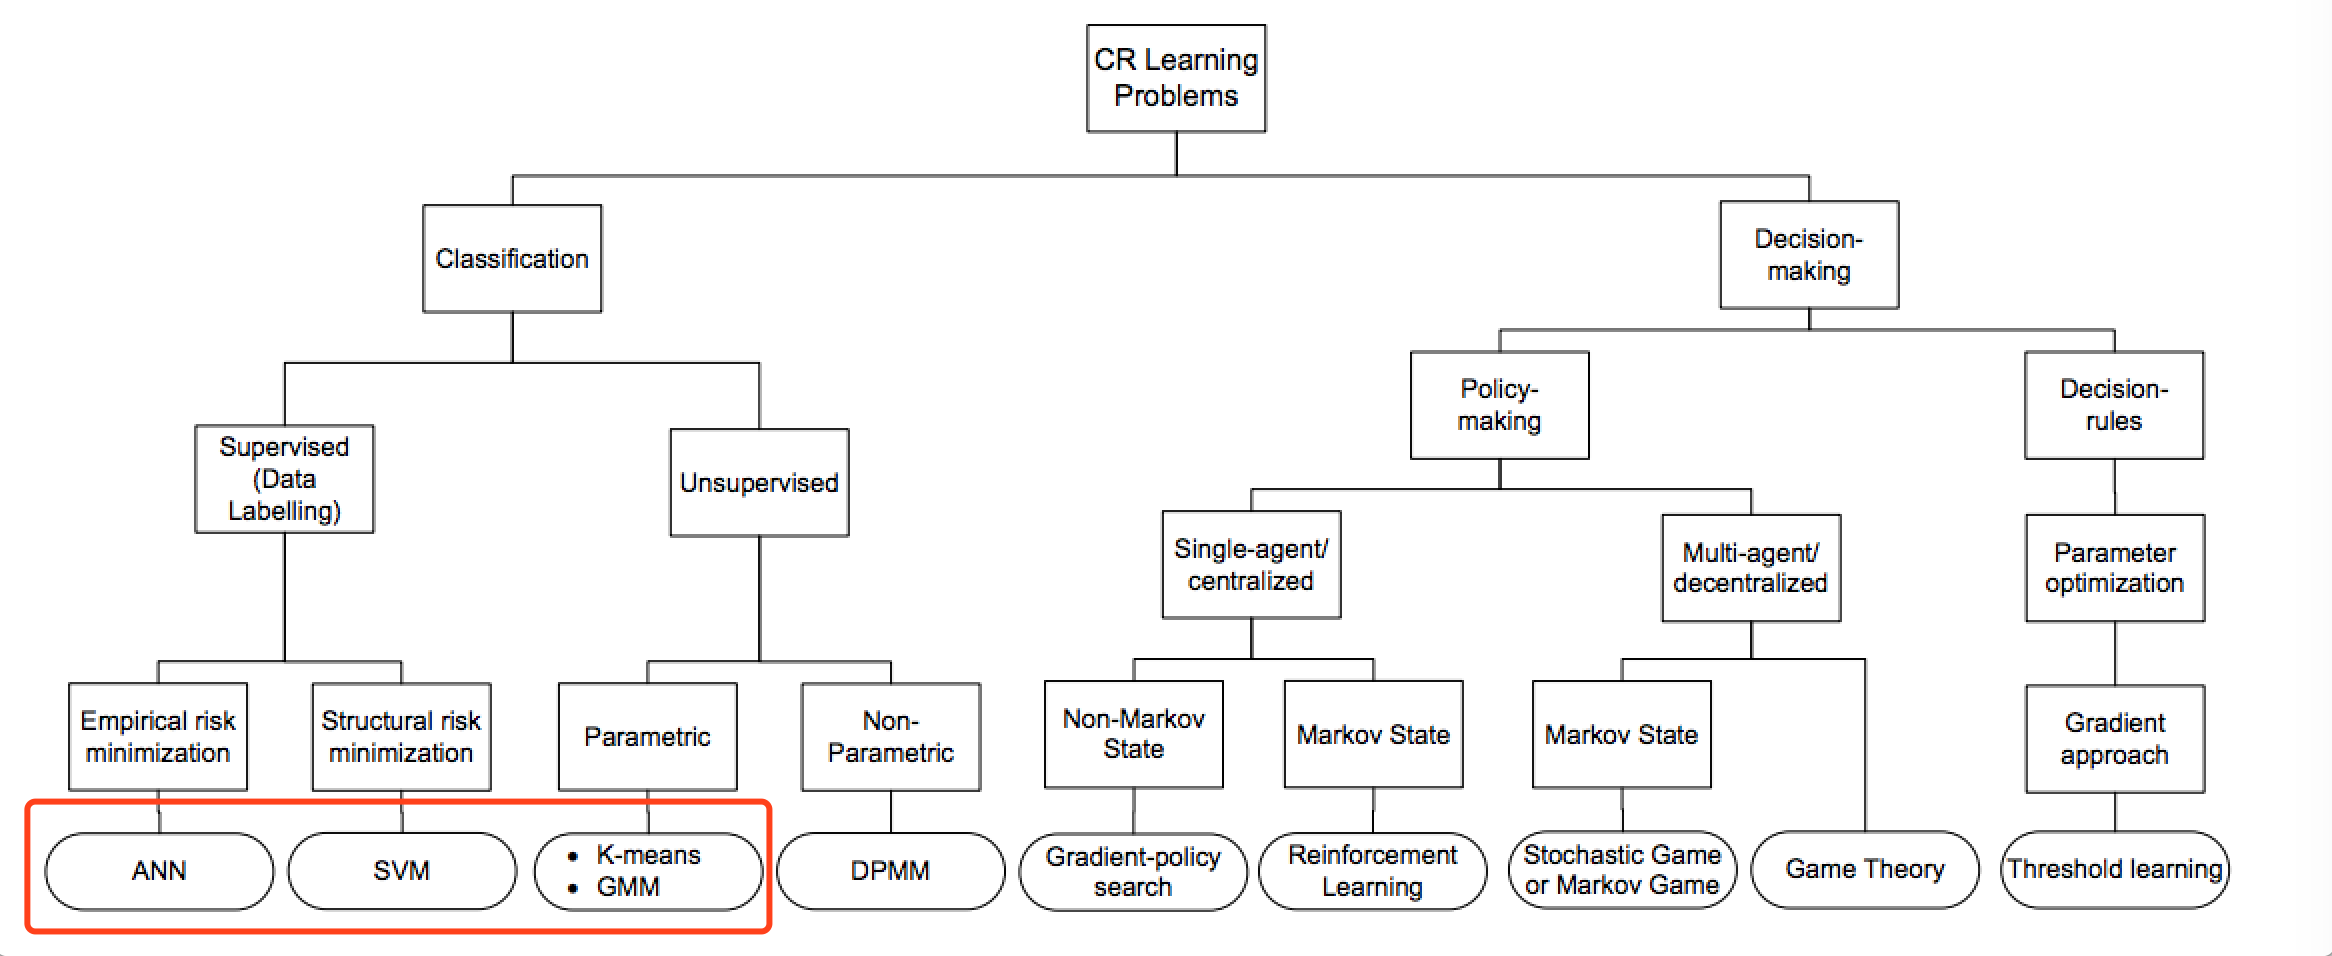
\includegraphics[width=0.8\textwidth]{CV_ML.png}

    \textsl{\caption{Typical problems in cognitive radio and their corresponding learning algorithms \cite{bkassiny2013survey}.}}
    \label{CognitiveCycle\&ML}
\end{figure*}
%\fi
Despite the numerous ML techniques, there are three main categories: supervised learning, unsupervised learning and reinforcement learning. One important criteria of whether an learning algorithm is supervised or unsupervised is the training set have target vector or not. According to \cite{nasrabadi2007pattern}, for supervised learning, the training process is based on the minimization of a loss function whereas there is no target vector for unsupervised learning. The goal is to find pattern or groups in the training set which is called clustering (i.e. K-means) or to find the distribution within the data, which is called density estimation (i.e. Gaussian Mixture Models (GMM)). Reinforcement learning is a technique learning what to do, that is, learning to map a situation observed by the interaction between agents and environment to maximize a reward function.
\subsection{Learning issue in CR}
From the perspective of machine learning, and according to previously introduced tasks of CR, learning problems can be classified as \cite{bkassiny2013survey}:

\begin{enumerate}
  \item Feature classification: spectrum hole detection, signal classification, etc.
  \item Decision-making: Parameters modification, adaptive modulation, power control, etc.
\end{enumerate}

It is crucial that allocating different tasks with appropriate learning algorithms. Fig.\ref{CognitiveCycle\&ML} summarized various state-of-the-art machine learning techniques with respect to CR learning problems. Supervised learning may be the best choice if CRs have prior knowledge about the environment. And unsupervised learning may the best choice for CR which operating in alien RF environment, under which case, autonomous unsupervised learning algorithms permit exploring the environment parameters and self-adapting without any prior knowledge.

For a single-agent CR, reinforcement learning is a good choice for CR operating under Markov process \cite{bkassiny2011distributed}, which will be introduced in the following section. The degree of freedom will be significantly increased when it comes to CRNs, the complex training process and considerably increased convergence time become the key issue.

Besides, regardless of what learning technique been employed, feature extraction lies at the heart of training a learning machine. Conventional signal classification schemes employ signal properties such as amplitude, frequency, and phase information to approach signal classification problems, which is time-consuming and baseband representation are required. Whereas, \cite{fehske2005new}  utilizes the cyclostationary signal feature, which is highly efficient, to solve such problem.

\subsection{Artificial Neural Network}
Artificial neural network (ANN) is a supervised learning algorithm, which does expect the prior knowledge of the observed environment. It is a promising technique for its adjustable architecture, remarkable nonlinear fitting and transfer learning properties for various tasks like convolutional neural network (CNN) for image classification, recurrent neural network (RNN) for sequence data with sequential information. \cite{tsagkaris2008neural} proposed an ANN scheme assisting CR to predict the data rate of selected radio parameters. And \cite{tumuluru2010neural} uses ANN to perform spectrum prediction for CR.

The architecture of a basic Artificial Neural Network (ANN) includes an input layer, a hidden layer, and an output layer \cite{schalkoff1997artificial}. Neurons communicate with each other by a weighted connection with bias. The sum of weighted outputs at each neuron is injected to a nonlinear activation function to get the output. There are several activation functions (i.e. ReLU, Sigmod) and the choice usually related to the problem to be solved.

Generally, the ANN is trained by gradient descent. Since mostly ANN has more than one hidden layer, then, it is time-consuming to calculate the gradient for each neuron even employed back-propagation (BP) algorithm to reduce the complexity of gradient descent. However, it can be optimized by transfer learning. The definition of transfer learning is given in \cite{pan2010survey}, given a source domain $\mathcal D_S$ and learning task $\mathcal T_S$ and a target domain $\mathcal D_T $ and learning task $\mathcal T_T$, transfer learning helps to improve the training of target function $f_T(\cdot)$ in $\mathcal D_T $ utilizing the knowledge of $\mathcal D_S$ and $\mathcal T_S$. Then, learning machine can be pre-trained based on previous knowledge of the RF environment before deploying.

\iffalse
\begin{figure}[!t]
    \centering
    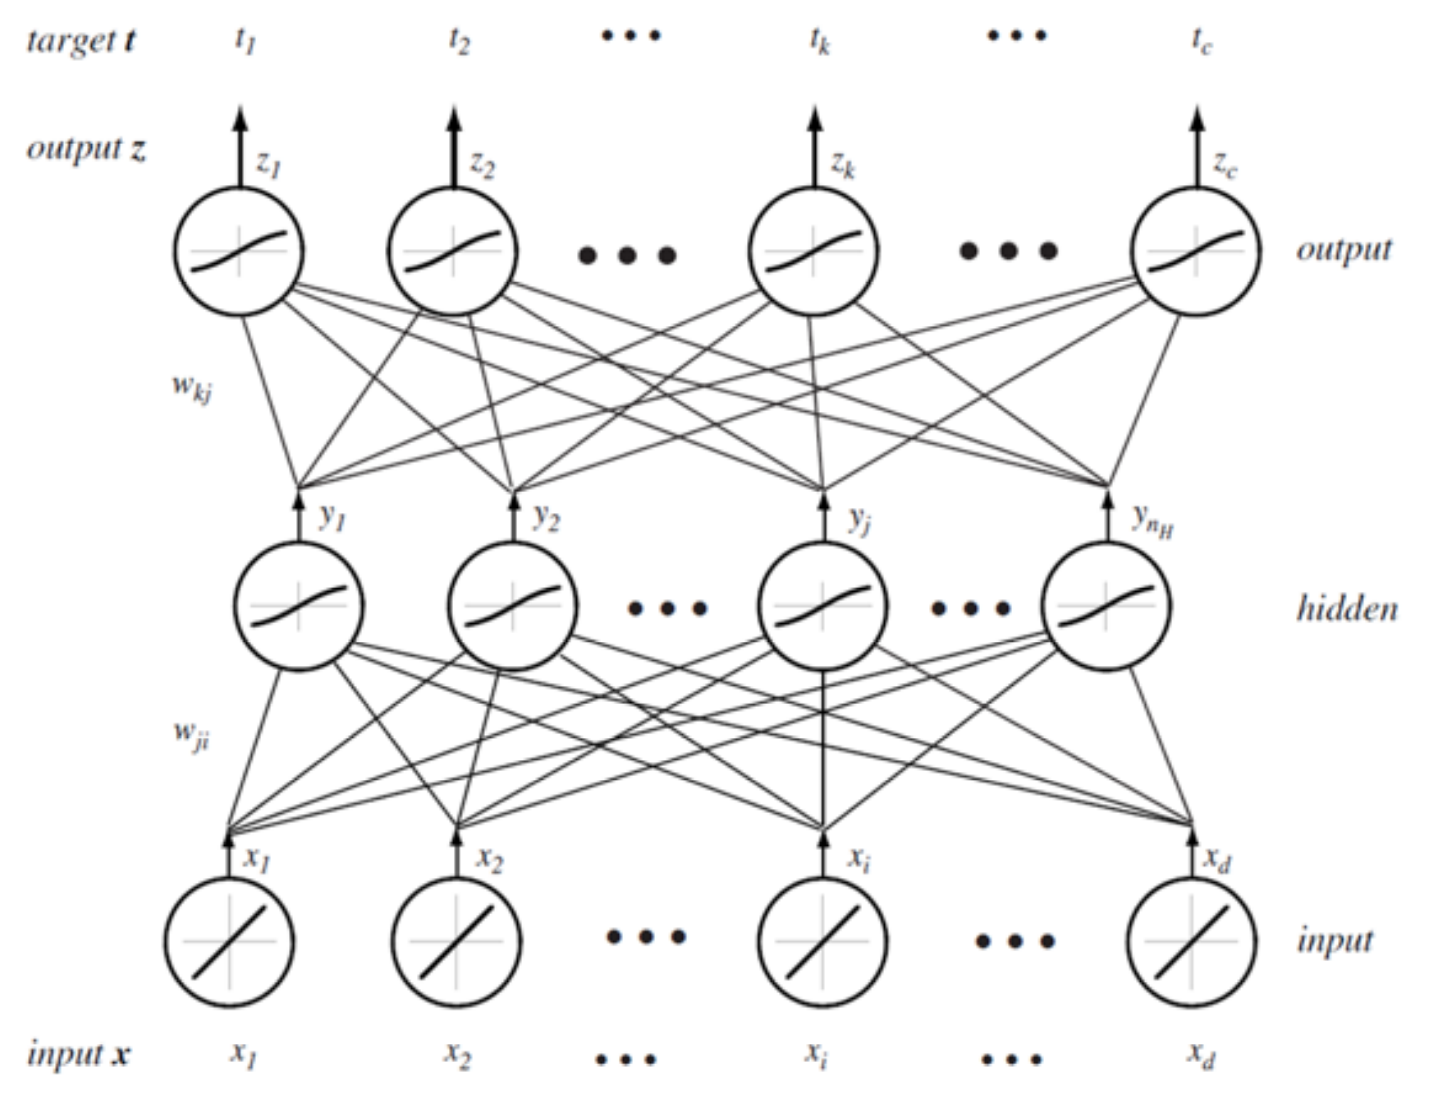
\includegraphics[width=2.2in]{ANN.png}
    \caption{Artifical Neural Network \cite{kate2017ANN}.}

\end{figure}
\fi
\subsection{Support Vector Machine for classification}
Support Vector Machine, sometimes called maximum margin classifier, is a famous supervised learning algorithm which used to solve classification problems. Basically, it can only solve binary classifications, but with some tricks (i.e. One-versus-One or One-versus-All), it can also handle multi-classification problems. Recently, SVM has been used for signal classification in cognitive radios \cite{hu2008signal}. It is a promising technique to solve classification problem for it maximum margin characteristic.

\subsection{Reinforcement learning for decision-making}
As noticed, reinforcement learning (RL) permits an agent/ learning machine to learn by interacting with the environment \cite{sutton1998reinforcement} without any prior knowledge, which is the key advantage of such technique because the nature of the radio frequency environment is unknown. Thus, this technique empowers the agent to learn without supervision. According to Fig.1, the decision-making process in CR is a process that enables CR to interact with the environment and such process can be improved by learning, thus making RL a promising choice for this task. RL has been used for dynamic spectrum access in cognitive radio network (CRN) \cite{yau2010applications}.

For each state $s_i$, a reinforcement learning machine have an action $a_i$ based on the actor/ policy $\pi_\theta (s)$, and got a reward from the environment $r_i$. The interaction process between learning machine and environment can be considered as a Markov decision process (MDP), where the state $s_{t+1}$ only determined by previous state $s_t$ and action $a_t$:
\begin{equation}
  p(s_{t+1}|s_t,a_t,s_{t-1},a_{t-1},...,s_{0},a_0) = p(s_{t+1}|s_t,a_t)
\end{equation}

For a given policy $\pi_\theta (s)$ and a given terminal state $s_T$, the trajectory of MDP is defined as $\tau = \{s_0,a_0,s_1,a_1,...,s_T,a_T\}$. The  cumulative reward $R(\tau)=\sum \limits_{n=1}^T r_n$ is what the training method need to maximize. And for those without terminal state, especially the case for cognitive radio, discounted future reward is defined as $R(\tau)=\sum \limits_{n=t}^T \gamma^{n-t}r_n$. Generally, the  cumulative reward $R(\tau)$ is a conditional random variable of policy $\pi_\theta$. The aim for training is to maximize the reward expection $\overline{R}_\theta$. However, conditional probability density function $p(\tau|\theta)$ is unreachable, where we use Monte Carlo method to approximate $\overline{R}_\theta$ by sampling. There are two ways in solving the problem under the assumption of Markov state, policy gradient and Q-learning. And gradient policy search is proposed for non-Markov state environment.



% An example of a floating figure using the graphicx package.
% Note that \label must occur AFTER (or within) \caption.
% For figures, \caption should occur after the \includegraphics.
% Note that IEEEtran v1.7 and later has special internal code that
% is designed to preserve the operation of \label within \caption
% even when the captionsoff option is in effect. However, because
% of issues like this, it may be the safest practice to put all your
% \label just after \caption rather than within \caption{}.
%
% Reminder: the "draftcls" or "draftclsnofoot", not "draft", class
% option should be used if it is desired that the figures are to be
% displayed while in draft mode.
%


% Note that IEEE typically puts floats only at the top, even when this
% results in a large percentage of a column being occupied by floats.


% An example of a double column floating figure using two subfigures.
% (The subfig.sty package must be loaded for this to work.)
% The subfigure \label commands are set within each subfloat command, the
% \label for the overall figure must come after \caption.
% \hfil must be used as a separator to get equal spacing.
% The subfigure.sty package works much the same way, except \subfigure is
% used instead of \subfloat.
%
%\begin{figure*}[!t]
%\centerline{\subfloat[Case I]\includegraphics[width=2.5in]{subfigcase1}%
%\label{fig_first_case}}
%\hfil
%\subfloat[Case II]{\includegraphics[width=2.5in]{subfigcase2}%
%\label{fig_second_case}}}
%\caption{Simulation results}
%\label{fig_sim}
%\end{figure*}
%
% Note that often IEEE papers with subfigures do not employ subfigure
% captions (using the optional argument to \subfloat), but instead will
% reference/describe all of them (a), (b), etc., within the main caption.


% An example of a floating table. Note that, for IEEE style tables, the
% \caption command should come BEFORE the table. Table text will default to
% \footnotesize as IEEE normally uses this smaller font for tables.
% The \label must come after \caption as always.
%
%\begin{table}[!t]
%% increase table row spacing, adjust to taste
%\renewcommand{\arraystretch}{1.3}
% if using array.sty, it might be a good idea to tweak the value of
% \extrarowheight as needed to properly center the text within the cells
%\caption{An Example of a Table}
%\label{table_example}
%\centering
%% Some packages, such as MDW tools, offer better commands for making tables
%% than the plain LaTeX2e tabular which is used here.
%\begin{tabular}{|c||c|}
%\hline
%One & Two\\
%\hline
%Three & Four\\
%\hline
%\end{tabular}
%\end{table}


% Note that IEEE does not put floats in the very first column - or typically
% anywhere on the first page for that matter. Also, in-text middle ("here")
% positioning is not used. Most IEEE journals use top floats exclusively.
% Note that, LaTeX2e, unlike IEEE journals, places footnotes above bottom
% floats. This can be corrected via the \fnbelowfloat command of the
% stfloats package.



\section{Conclusion}
As a promising technique of opportunistic spectrum access, the scheme and tasks of cognitive radio have been present. Besides, this review characteristic the learning problem in CR to achieve the understanding-by-building goal, which can be greatly assisted by machine learning technique due to their inherent learning by observing property.

Besides, some promising learning technique like ANN, SVM, and reinforcement learning have been introduced to solve the supervised and unsupervised learning problems in familiar and alien RF environment, which technique can be used to solve different tasks with respect superiorities. The main considerations for the application of ML to CR in the future are the convergence time, implementation complexity and robustness of the system. Despite the fact that there do have an increasing number of applications of ML to cognitive radio but such applications are still not complete and have tremendous potential to be explored. What's more, feature extraction always significantly contributes to the accuracy and efficiency of learning machine regardless of which algorithm been employed.

Apart from ML technique, under the circumstance of cognitive radio networks, game theory provides analytical tools to acquire interaction among users and makes such problem analytically tractable, which should be considered in the future work.



% if have a single appendix:
%\appendix[Proof of the Zonklar Equations]
% or
%\appendix  % for no appendix heading
% do not use \section anymore after \appendix, only \section*
% is possibly needed

% use appendices with more than one appendix
% then use \section to start each appendix
% you must declare a \section before using any
% \subsection or using \label (\appendices by itself
% starts a section numbered zero.)
%



% trigger a \newpage just before the given reference
% number - used to balance the columns on the last page
% adjust value as needed - may need to be readjusted if
% the document is modified later
%\IEEEtriggeratref{8}
% The "triggered" command can be changed if desired:
%\IEEEtriggercmd{\enlargethispage{-5in}}

% references section

% can use a bibliography generated by BibTeX as a .bbl file
% BibTeX documentation can be easily obtained at:
% http://www.ctan.org/tex-archive/biblio/bibtex/contrib/doc/
% The IEEEtran BibTeX style support page is at:
% http://www.michaelshell.org/tex/ieeetran/bibtex/
%\bibliographystyle{IEEEtran}
% argument is your BibTeX string definitions and bibliography database(s)
%\bibliography{IEEEabrv,../bib/paper}
%
% <OR> manually copy in the resultant .bbl file
% set second argument of \begin to the number of references
% (used to reserve space for the reference number labels box)

% biography section
%
% If you have an EPS/PDF photo (graphicx package needed) extra braces are
% needed around the contents of the optional argument to biography to prevent
% the LaTeX parser from getting confused when it sees the complicated
% \includegraphics command within an optional argument. (You could create
% your own custom macro containing the \includegraphics command to make things
% simpler here.)
%\begin{biography}[{\includegraphics[width=1in,height=1.25in,clip,keepaspectratio]{mshell}}]{Michael Shell}
% or if you just want to reserve a space for a photo:

% You can push biographies down or up by placing
% a \vfill before or after them. The appropriate
% use of \vfill depends on what kind of text is
% on the last page and whether or not the columns
% are being equalized.

%\vfill

% Can be used to pull up biographies so that the bottom of the last one
% is flush with the other column.
%\enlargethispage{-5in}


%\bibliographystyle{ieeetr}
%\bibliography{cite}
%\scriptsize
\begin{thebibliography}{10}
\scriptsize
\bibitem{mitola1999cognitive}
J.~Mitola and G.~Q. Maguire, ``Cognitive radio: making software radios more
  personal,'' {\em IEEE personal communications}, vol.~6, no.~4, pp.~13--18,
  1999.

\bibitem{haykin2005cognitive}
S.~Haykin, ``Cognitive radio: brain-empowered wireless communications,'' {\em
  IEEE journal on selected areas in communications}, vol.~23, no.~2,
  pp.~201--220, 2005.

\bibitem{bkassiny2013survey}
M.~Bkassiny, Y.~Li, and S.~K. Jayaweera, ``A survey on machine-learning
  techniques in cognitive radios,'' {\em IEEE Communications Surveys \&
  Tutorials}, vol.~15, no.~3, pp.~1136--1159, 2013.

\bibitem{mchenry2006chicago}
M.~A. McHenry, P.~A. Tenhula, D.~McCloskey, D.~A. Roberson, and C.~S. Hood,
  ``Chicago spectrum occupancy measurements \& analysis and a long-term studies
  proposal,'' in {\em Proceedings of the first international workshop on
  Technology and policy for accessing spectrum}, p.~1, ACM, 2006.

\bibitem{islam2008spectrum}
M.~H. Islam, C.~L. Koh, S.~W. Oh, X.~Qing, Y.~Y. Lai, C.~Wang, Y.-C. Liang,
  B.~E. Toh, F.~Chin, G.~L. Tan, {\em et~al.}, ``Spectrum survey in singapore:
  Occupancy measurements and analyses,'' in {\em Cognitive Radio Oriented
  Wireless Networks and Communications, 2008. CrownCom 2008. 3rd International
  Conference on}, pp.~1--7, IEEE, 2008.

\bibitem{he2010survey}
A.~He, K.~K. Bae, T.~R. Newman, J.~Gaeddert, K.~Kim, R.~Menon,
  L.~Morales-Tirado, Y.~Zhao, J.~H. Reed, W.~H. Tranter, {\em et~al.}, ``A
  survey of artificial intelligence for cognitive radios,'' {\em IEEE
  Transactions on Vehicular Technology}, vol.~59, no.~4, pp.~1578--1592, 2010.

\bibitem{jayaweera2011radiobots}
S.~Jayaweera and C.~Christodoulou, ``Radiobots: Architecture, algorithms and
  realtime reconfigurable antenna designs for autonomous, self-learning future
  cognitive radios,'' 2011.

\bibitem{nasrabadi2007pattern}
N.~M. Nasrabadi, ``Pattern recognition and machine learning,'' {\em Journal of
  electronic imaging}, vol.~16, no.~4, p.~049901, 2007.

\bibitem{bkassiny2011distributed}
M.~Bkassiny, S.~K. Jayaweera, and K.~A. Avery, ``Distributed reinforcement
  learning based mac protocols for autonomous cognitive secondary users,'' in
  {\em Wireless and Optical Communications Conference (WOCC), 2011 20th
  Annual}, pp.~1--6, IEEE, 2011.

\bibitem{fehske2005new}
A.~Fehske, J.~Gaeddert, and J.~H. Reed, ``A new approach to signal
  classification using spectral correlation and neural networks,'' in {\em New
  Frontiers in Dynamic Spectrum Access Networks, 2005. DySPAN 2005. 2005 First
  IEEE International Symposium on}, pp.~144--150, IEEE, 2005.

\bibitem{tsagkaris2008neural}
K.~Tsagkaris, A.~Katidiotis, and P.~Demestichas, ``Neural network-based
  learning schemes for cognitive radio systems,'' {\em Computer
  Communications}, vol.~31, no.~14, pp.~3394--3404, 2008.

\bibitem{tumuluru2010neural}
V.~K. Tumuluru, P.~Wang, and D.~Niyato, ``A neural network based spectrum
  prediction scheme for cognitive radio,'' in {\em Communications (ICC), 2010
  IEEE International Conference on}, pp.~1--5, IEEE, 2010.

\bibitem{schalkoff1997artificial}
R.~J. Schalkoff, {\em Artificial neural networks}, vol.~1.
\newblock McGraw-Hill New York, 1997.

\bibitem{pan2010survey}
S.~J. Pan and Q.~Yang, ``A survey on transfer learning,'' {\em IEEE
  Transactions on knowledge and data engineering}, vol.~22, no.~10,
  pp.~1345--1359, 2010.

\bibitem{hu2008signal}
H.~Hu, Y.~Wang, and J.~Song, ``Signal classification based on spectral
  correlation analysis and svm in cognitive radio,'' in {\em Advanced
  Information Networking and Applications, 2008. AINA 2008. 22nd International
  Conference on}, pp.~883--887, IEEE, 2008.

\bibitem{sutton1998reinforcement}
R.~S. Sutton and A.~G. Barto, {\em Reinforcement learning: An introduction},
  vol.~1.
\newblock MIT press Cambridge, 1998.

\bibitem{yau2010applications}
K.-L.~A. Yau, P.~Komisarczuk, and P.~D. Teal, ``Applications of reinforcement
  learning to cognitive radio networks,'' in {\em Communications Workshops
  (ICC), 2010 IEEE International Conference on}, pp.~1--6, IEEE, 2010.

\end{thebibliography}

% that's all folks

\end{document}
